\documentclass[conference]{IEEEtran}
\IEEEoverridecommandlockouts

% ── Packages ──────────────────────────────────────────────────────────────────
\usepackage{cite}
\usepackage{amsmath,amssymb}
\usepackage{algorithmic}
\usepackage{algorithm}
\usepackage{graphicx}
\usepackage{xcolor}
\usepackage{tikz}
\usepackage{listings}
\usepackage{placeins}
\usetikzlibrary{positioning, arrows.meta, shapes.geometric, shadows}

\renewcommand{\algorithmicrequire}{\textbf{Input:}}
\renewcommand{\algorithmicensure}{\textbf{Output:}}

% ── JSON listing style ────────────────────────────────────────────────────────
\definecolor{jsonkey}{RGB}{163,21,21}
\definecolor{jsonstring}{RGB}{0,128,0}
\definecolor{jsonnumber}{RGB}{0,0,205}
\lstdefinelanguage{json}{
  basicstyle=\ttfamily\scriptsize,
  columns=fullflexible,
  showstringspaces=false,
  commentstyle=\color{gray},
  string=[s]{"}{"},
  stringstyle=\color{jsonstring},
  literate=
    *{0}{{{\color{jsonnumber}0}}}{1}
     {1}{{{\color{jsonnumber}1}}}{1}
     {2}{{{\color{jsonnumber}2}}}{1}
     {3}{{{\color{jsonnumber}3}}}{1}
     {4}{{{\color{jsonnumber}4}}}{1}
     {5}{{{\color{jsonnumber}5}}}{1}
     {6}{{{\color{jsonnumber}6}}}{1}
     {7}{{{\color{jsonnumber}7}}}{1}
     {8}{{{\color{jsonnumber}8}}}{1}
     {9}{{{\color{jsonnumber}9}}}{1}
     {:}{{{\color{jsonkey}{:}}}}{1}
     {,}{{{\color{black}{,}}}}{1}
     {\{}{{{\color{black}{\{}}}}{1}
     {\}}{{{\color{black}{\}}}}}{1}
     {[}{{{\color{black}{[}}}}{1}
     {]}{{{\color{black}{]}}}}{1},
}

% ══════════════════════════════════════════════════════════════════════════════
\begin{document}

\title{Plague Containment}

\author{
  \IEEEauthorblockN{Nelson David Molina Ramos}
  \IEEEauthorblockA{\textit{Computer Engineering Program}\\
    Universidad Distrital Francisco Jos\'{e} de Caldas\\
    Bogot\'{a}, Colombia}
  \and
  \IEEEauthorblockN{Brayan Estiven Aguirre Aristizabal}
  \IEEEauthorblockA{\textit{Computer Engineering Program}\\
    Universidad Distrital Francisco Jos\'{e} de Caldas\\
    Bogot\'{a}, Colombia}
  \and
  \IEEEauthorblockN{Juan Sneyder M\'{e}ndez Gil}
  \IEEEauthorblockA{\textit{Computer Engineering Program}\\
    Universidad Distrital Francisco Jos\'{e} de Caldas\\
    Bogot\'{a}, Colombia}
}

\maketitle

% ── Abstract ──────────────────────────────────────────────────────────────────
\begin{abstract}
This paper describes the design of Plague Containment, an interactive grid-based
strategy game developed as part of the Computer Sciences~I course project. The
game models a city as an $8\times8$ grid of districts, each with a different
infection risk level. The player must stop a spreading plague using two
algorithmic tools: a greedy vaccination strategy, which always targets the
highest-risk uninfected district bordering the infection, and a backtracking
quarantine planner, which looks for a ring of districts that encloses the
infected zone without cutting off any healthy part of the city. This paper
presents the problem background, the city model, the design of both algorithms
through pseudo-code, the JSON communication schema that bridges the C++ engine
with the Python algorithms and the Pygame interface, and a wireframe of the
game screen.
\end{abstract}

\begin{IEEEkeywords}
greedy algorithm, backtracking, epidemic containment, grid model, game design,
algorithm design, system integration, JSON bridge.
\end{IEEEkeywords}

% ══════════════════════════════════════════════════════════════════════════════
\section{Introduction}

Plague Containment is a turn-based strategy game that puts the player in charge
of stopping an outbreak across a city grid. Each district has an infection risk
level, and the plague spreads every turn to neighbor districts. The player has
two tools: vaccinate a district to make it immune, or establish a quarantine
perimeter to isolate the infected zone.

Two algorithms assist the player. The greedy advisor scans the border of the
infected zone and recommends the healthy district with the highest-risk to
vaccinate. The backtracking algorithm searches for a valid quarantine ring that
surrounds all infected districts while ensuring no healthy district becomes cut
off from the rest of the city.

The goal of this paper is to describe the city model, present the design and
pseudo-code of both algorithms, define the JSON schema that connects the three
system layers, and show the wireframe of the game interface.

% ══════════════════════════════════════════════════════════════════════════════
\section{City Grid Model}

\subsection{The Grid}

The city is represented as an $8\times8$ grid of districts. Each cell in the
grid corresponds to one district. Two districts are considered neighbors if they
share a side (up, down, left, right).

\subsection{District States}

Every district is always in exactly one of four possible states:

\begin{itemize}
  \item \textbf{Healthy} — not yet affected by the plague.
  \item \textbf{Infected} — currently carrying the plague and
        spreading it to neighbors.
  \item \textbf{Vaccinated} — immunized by the player; cannot
        become infected.
  \item \textbf{Quarantined} — placed under lockdown by the
        backtracking planner to form the containment perimeter.
\end{itemize}

\subsection{Risk Level}

Each district has a risk level, which is a whole number between 1 and 10
assigned at the start of the game. A higher risk level means that the district
is more vulnerable to contracting the plague (for example, due to high
population density or poor sanitation). The risk level does not change during
the game.

\subsection{How the Plague Spreads}

At the end of each turn, the plague attempts to spread. For every infected
district, each of its healthy neighbors has a chance of becoming infected.
Districts that are vaccinated or quarantined block the spread entirely.

Figure~\ref{fig:grid} shows an example of the grid mid-game.

\begin{figure}[h]
    \centering
    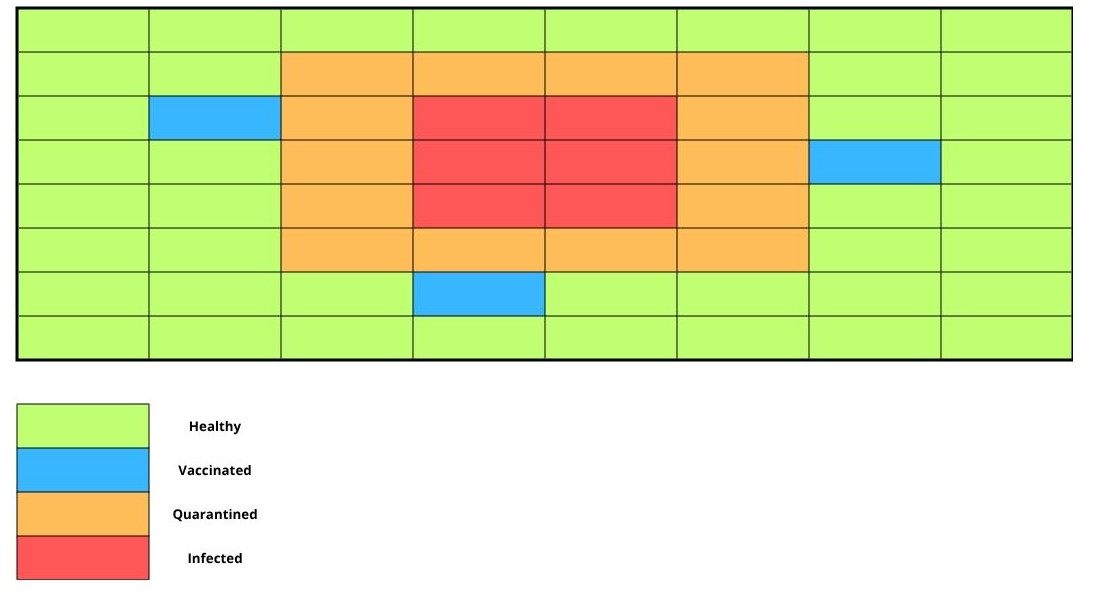
\includegraphics[width=0.5\textwidth]{f1.jpg}
    \caption{Example of the grid mid-game}
    \label{fig:grid}
\end{figure}

% ══════════════════════════════════════════════════════════════════════════════
\section{Greedy Vaccination Algorithm}

\subsection{What It Does}

The greedy algorithm helps the player decide which district to vaccinate on
each turn. It works by looking at every healthy district that directly borders
an infected one, and recommending the one with the highest risk level. The idea
is simple: vaccinate the most dangerous unprotected neighbor before the plague
reaches it.

\subsection{Why Greedy Works Here}

Greedy algorithms are a good fit when each decision can be made locally without
looking far ahead. In this case, the most urgent district to protect is always
the one most likely to spread the plague further — which is the one with the
highest risk. The greedy choice aligns directly with the immediate threat.

\subsection{Pseudo-code}

\begin{algorithm}[ht]
\caption{Greedy Vaccination}
\label{alg:greedy}
\begin{algorithmic}[1]
\REQUIRE The game grid with all district states and risk levels
\ENSURE The best district to vaccinate this turn, or None

\STATE $\mathit{candidates} \leftarrow$ empty list
\FOR{each infected district $d$ on the grid}
  \FOR{each neighbor $n$ of $d$}
    \IF{$n$ is \textsc{healthy}}
      \STATE add $n$ to $\mathit{candidates}$ (avoid duplicates)
    \ENDIF
  \ENDFOR
\ENDFOR

\IF{$\mathit{candidates}$ is empty}
  \RETURN \textsc{None}
\ENDIF

\STATE $\mathit{best} \leftarrow$ first district in $\mathit{candidates}$
\FOR{each district $c$ in $\mathit{candidates}$}
  \IF{$c.\mathit{risk} > \mathit{best}.\mathit{risk}$}
    \STATE $\mathit{best} \leftarrow c$
  \ENDIF
\ENDFOR

\STATE mark $\mathit{best}$ as \textsc{vaccinated}
\RETURN $\mathit{best}$
\end{algorithmic}
\end{algorithm}

% ══════════════════════════════════════════════════════════════════════════════
\section{Backtracking Quarantine Algorithm}

\subsection{What It Does}

The backtracking algorithm finds a set of healthy districts to quarantine so
that the infected zone is completely enclosed. The result must satisfy two
conditions at the same time:

\begin{enumerate}
  \item \textbf{Full enclosure.} Every infected district must be
        completely surrounded — none of its neighbors can remain
        a free healthy district.
  \item \textbf{No isolation.} After quarantine is placed, every
        healthy district that is not quarantined must still be
        reachable from the rest of the healthy city. No healthy
        area can become a disconnected island.
\end{enumerate}

\subsection{Why Backtracking}

This is not a greedy problem because a locally good choice can create a
globally bad outcome. For instance, quarantining a district that seems necessary might accidentally cut off a healthy neighborhood. Backtracking allows the algorithm to try a choice, check if both conditions are met, and undo that choice if they are not — exploring alternatives until a valid solution is found.

\subsection{Pseudocode}

Algorithm~\ref{alg:bt_main} is the starting point.
Algorithm~\ref{alg:bt_worker} is the recursive function it calls.

\begin{algorithm}[H]
\caption{Backtracking Quarantine — Entry Point}
\label{alg:bt_main}
\begin{algorithmic}[1]
\REQUIRE The game grid with all district states
\ENSURE A valid quarantine set, or \textsc{None} if impossible

\STATE $\mathit{border} \leftarrow$ all healthy neighbors of infected districts
\STATE $\mathit{quarantine} \leftarrow$ empty set
\STATE $\mathit{success} \leftarrow$
       \textsc{Search}($\mathit{border}$, index $0$, $\mathit{quarantine}$)
\IF{$\mathit{success}$}
  \RETURN $\mathit{quarantine}$
\ELSE
  \RETURN \textsc{None}
\ENDIF
\end{algorithmic}
\end{algorithm}
\vspace{-5pt}
\begin{algorithm}[H]
\caption{Search — Recursive Backtracking Step}
\label{alg:bt_worker}
\begin{algorithmic}[1]
\REQUIRE Border district list, current index $i$,
         partial quarantine set $\mathit{quarantine}$
\ENSURE \textsc{True} if a complete valid quarantine was found,
        \textsc{False} otherwise

\IF{infected zone is fully enclosed by $\mathit{quarantine}$}
  \RETURN \textsc{True}
  \COMMENT{Both conditions satisfied — solution found}
\ENDIF

\IF{no more border districts to try}
  \RETURN \textsc{False}
  \COMMENT{Ran out of candidates without full enclosure}
\ENDIF

\STATE $d \leftarrow \mathit{border}[i]$

\COMMENT{--- Option A: quarantine district $d$ ---}
\STATE add $d$ to $\mathit{quarantine}$
\STATE temporarily mark $d$ as \textsc{quarantined} on the grid

\IF{remaining healthy districts are still all connected}
  \IF{\textsc{Search}($\mathit{border}$, $i+1$, $\mathit{quarantine}$)}
    \RETURN \textsc{True}
  \ENDIF
\ENDIF

\COMMENT{--- Backtrack: undo quarantine of $d$ ---}
\STATE remove $d$ from $\mathit{quarantine}$
\STATE restore $d$ to \textsc{healthy} on the grid

\COMMENT{--- Option B: skip district $d$ ---}
\IF{\textsc{Search}($\mathit{border}$, $i+1$, $\mathit{quarantine}$)}
  \RETURN \textsc{True}
\ENDIF

\RETURN \textsc{False}
\end{algorithmic}
\end{algorithm}
% ══════════════════════════════════════════════════════════════════════════════
\section{How the Two Algorithms Work Together}

The greedy and backtracking algorithms serve different roles during a game
turn. Figure~\ref{fig:loop} shows the sequence of events within a single turn.

\begin{figure}[H]
\centering
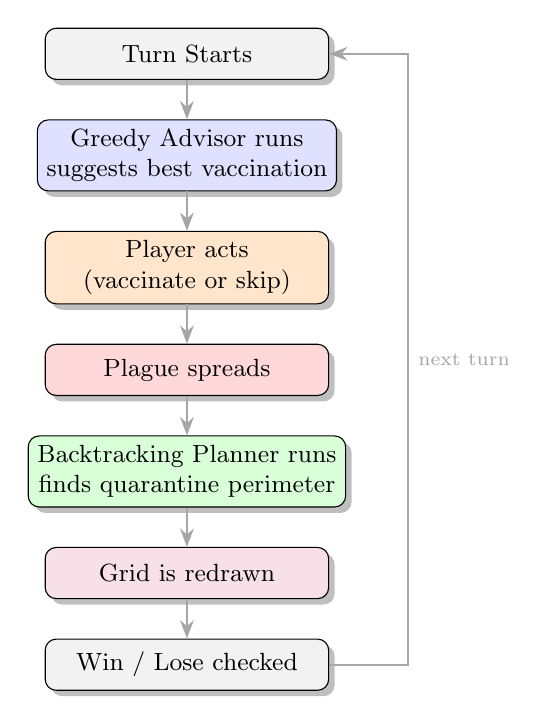
\begin{tikzpicture}[
  box/.style={draw, rounded corners=4pt, minimum width=3.6cm,
              minimum height=0.65cm, align=center, font=\small,
              fill=white, drop shadow},
  arr/.style={-Stealth, thick, gray!70}
]
  \node[box, fill=gray!10]   (start)  {Turn Starts};
  \node[box, fill=blue!12,   below=0.5cm of start]  (greedy)
    {Greedy Advisor runs\\suggests best vaccination};
  \node[box, fill=orange!20, below=0.5cm of greedy] (player)
    {Player acts\\(vaccinate or skip)};
  \node[box, fill=red!15,    below=0.5cm of player] (spread)
    {Plague spreads};
  \node[box, fill=green!15,  below=0.5cm of spread] (bt)
    {Backtracking Planner runs\\finds quarantine perimeter};
  \node[box, fill=purple!12, below=0.5cm of bt]     (render)
    {Grid is redrawn};
  \node[box, fill=gray!10,   below=0.5cm of render] (check)
    {Win / Lose checked};

  \draw[arr] (start)  -- (greedy);
  \draw[arr] (greedy) -- (player);
  \draw[arr] (player) -- (spread);
  \draw[arr] (spread) -- (bt);
  \draw[arr] (bt)     -- (render);
  \draw[arr] (render) -- (check);
  \draw[arr] (check.east) -- ++(1.0,0) |- (start.east)
    node[pos=0.25, right, font=\scriptsize] {next turn};
\end{tikzpicture}
\caption{Sequence of events inside one game turn.}
\label{fig:loop}
\end{figure}

The greedy algorithm runs quickly and gives the player a recommendation
\emph{before} they act. The backtracking planner runs \emph{after} the plague spreads so that the displayed quarantine perimeter always reflects the current state of the grid.

% ══════════════════════════════════════════════════════════════════════════════
\section{System Architecture and Integration}

The Plague Containment game is built on a three-layer architecture in which
each layer is implemented in a different language. The C++ engine manages the
core data structures (the infection linked list and the district AVL tree). The
Python layer implements the greedy and backtracking algorithms. The Pygame
module renders the graphical interface and captures user input. These three
layers do not call each other directly; instead, they communicate through a
shared JSON file that acts as a language-neutral bridge.

\subsection{Why a JSON Bridge?}

C++ and Python are compiled and interpreted languages, respectively, and mixing
them via direct bindings (e.g.\ \texttt{pybind11}) adds complexity beyond the
scope of this course. A JSON file provides a simple, human-readable interface
that both languages can read and write using their standard libraries
(\texttt{nlohmann/json} in C++, \texttt{json} in Python). This also makes
debugging straightforward: at any point during development, a team member can
open the JSON file and inspect the full game state.

\subsection{Component Responsibilities}

Table~\ref{tab:components} summarizes what each component owns.

\begin{table}[ht]
\centering
\caption{Responsibility of each system component.}
\label{tab:components}
\begin{tabular}{|p{1.4cm}|p{2.0cm}|p{4.0cm}|}
\hline
\textbf{Layer} & \textbf{Language} & \textbf{Responsibilities} \\
\hline
Engine &
C++ &
Maintain the infection chain (linked list) and district risk index (AVL tree).
Update plague spread each turn. Write the updated game state to JSON. \\
\hline
Algorithms &
Python &
Read the game state from JSON. Run the greedy advisor and the backtracking
planner. Write algorithm results (recommendation, quarantine set) back to
JSON. \\
\hline
Interface &
Python / Pygame &
Read the game state and algorithm results from JSON. Render the grid,
highlights, and HUD. Capture player input and write the chosen action to
JSON. \\
\hline
\end{tabular}
\end{table}

\subsection{Communication Flow}

Figure~\ref{fig:dataflow} illustrates how data moves through the system during
a single game turn.

\begin{figure}[ht]
\centering
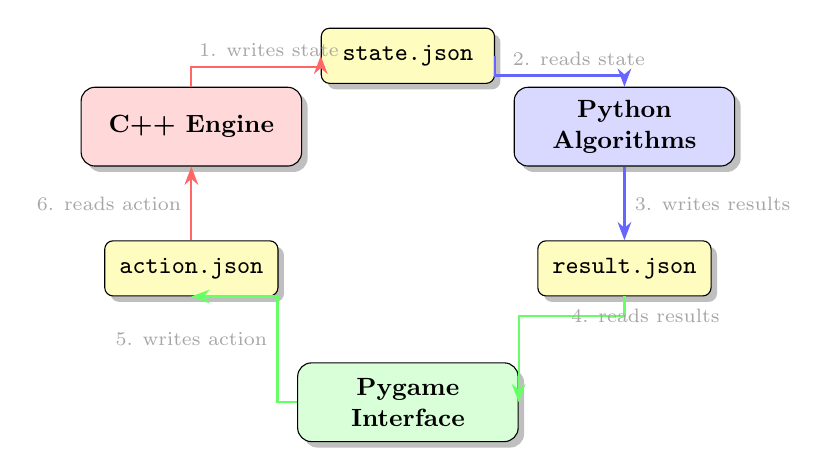
\begin{tikzpicture}[
  component/.style={draw, rounded corners=5pt, minimum width=2.8cm,
              minimum height=1.0cm, align=center, font=\small\bfseries,
              drop shadow},
  jsonbox/.style={draw, rounded corners=3pt, minimum width=2.2cm,
              minimum height=0.7cm, align=center, font=\small,
              fill=yellow!25, drop shadow},
  arr/.style={-Stealth, thick},
  note/.style={font=\scriptsize, text=gray!70}
]

  % Components
  \node[component, fill=red!15]    (cpp)  at (0, 0)      {C++ Engine};
  \node[component, fill=blue!15]   (py)   at (5.5, 0)    {Python\\Algorithms};
  \node[component, fill=green!15]  (ui)   at (2.75, -3.5){Pygame\\Interface};

  % JSON nodes
  \node[jsonbox] (json1) at (2.75, 0.9)  {\texttt{state.json}};
  \node[jsonbox] (json2) at (5.5, -1.8)  {\texttt{result.json}};
  \node[jsonbox] (json3) at (0, -1.8)    {\texttt{action.json}};

  % Arrows
  \draw[arr, red!60]   (cpp.north) -- ++(0,0.25) -| (json1.west)
    node[pos=0.3, above, note] {1. writes state};
  \draw[arr, blue!60]  (json1.east) |- ++(0.2,-0.25) -| (py.north)
    node[pos=0.3, above, note] {2. reads state};
  \draw[arr, blue!60]  (py.south) -- (json2.north)
    node[pos=0.5, right, note] {3. writes results};
  \draw[arr, green!60] (json2.south) -- ++(0,-0.25) -| (ui.east)
    node[pos=0.3, right, note] {4. reads results};
  \draw[arr, green!60] (ui.west) -- ++(-0.25,0) |- (json3.south)
    node[pos=0.3, left, note] {5. writes action};
  \draw[arr, red!60]   (json3.north) -- (cpp.south)
    node[pos=0.5, left, note] {6. reads action};

\end{tikzpicture}
\caption{Data flow between the three system components through JSON files.
Numbers indicate the order within one turn.}
\label{fig:dataflow}
\end{figure}

The cycle works as follows:

\begin{enumerate}
    \item The \textbf{C++ engine} updates the game state (plague spread, data
          structures) and writes the result to \texttt{state.json}.
    \item The \textbf{Python algorithm module} reads \texttt{state.json}, runs
          the greedy advisor and the backtracking planner, and writes its
          recommendations to \texttt{result.json}.
    \item The \textbf{Pygame interface} reads both files, renders the grid with
          the algorithm suggestions highlighted, and waits for the player to
          act.
    \item When the player clicks, the interface writes the chosen action to
          \texttt{action.json}.
    \item The \textbf{C++ engine} reads \texttt{action.json}, applies the
          action (e.g.\ vaccinate a district), advances the turn, and the
          cycle repeats.
\end{enumerate}

% ══════════════════════════════════════════════════════════════════════════════
\section{JSON Schema Design}

Three JSON files mediate all inter-component communication. This section
defines the structure of each one.

\subsection{Game State (\texttt{state.json})}

This file is written by the C++ engine and read by both Python and Pygame. It
contains the complete snapshot of the game at the start of a turn.

\begin{lstlisting}[language=json, frame=single,
  caption={Example \texttt{state.json} (turn 3).},
  label={lst:state}]
{
  "turn": 3,
  "grid_size": 8,
  "districts": [
    {
      "row": 0, "col": 0,
      "risk": 5,
      "state": "healthy"
    },
    {
      "row": 0, "col": 1,
      "risk": 8,
      "state": "infected"
    },
    {
      "row": 1, "col": 0,
      "risk": 3,
      "state": "vaccinated"
    },
    {
      "row": 1, "col": 1,
      "risk": 7,
      "state": "quarantined"
    }
  ],
  "infection_chain": [
    {"row": 3, "col": 4, "turn_infected": 1},
    {"row": 3, "col": 5, "turn_infected": 1},
    {"row": 2, "col": 4, "turn_infected": 2},
    {"row": 4, "col": 4, "turn_infected": 3}
  ],
  "stats": {
    "total_infected": 4,
    "total_vaccinated": 6,
    "total_quarantined": 2,
    "total_healthy": 52
  }
}
\end{lstlisting}

Key design decisions:

\begin{itemize}
    \item Each district is identified by its \texttt{(row, col)} pair, which
          maps directly to a grid cell.
    \item The \texttt{state} field uses one of four string values:
          \texttt{"healthy"}, \texttt{"infected"}, \texttt{"vaccinated"}, or
          \texttt{"quarantined"}.
    \item The \texttt{infection\_chain} array mirrors the linked list
          maintained by C++. It preserves insertion order so that Python and
          Pygame can reconstruct the chronological spread of the plague.
    \item The \texttt{stats} object provides precomputed counters so that the
          interface can display them without iterating over the full grid.
\end{itemize}

\subsection{Algorithm Results (\texttt{result.json})}

This file is written by the Python algorithm module after processing the game
state. It contains the greedy recommendation and the backtracking quarantine
plan.

\begin{lstlisting}[language=json, frame=single,
  caption={Example \texttt{result.json}.},
  label={lst:result}]
{
  "greedy_recommendation": {
    "row": 2, "col": 5,
    "risk": 9,
    "reason": "highest-risk healthy neighbor"
  },
  "quarantine_plan": {
    "found": true,
    "districts": [
      {"row": 2, "col": 3},
      {"row": 4, "col": 5},
      {"row": 5, "col": 4},
      {"row": 3, "col": 6}
    ],
    "cost": 4
  }
}
\end{lstlisting}

If the backtracking algorithm cannot find a valid quarantine, the
\texttt{found} field is set to \texttt{false} and the \texttt{districts} array
is empty.

\subsection{Player Action (\texttt{action.json})}

This file is written by the Pygame interface when the player makes a decision
and is read by the C++ engine to apply the change.

\begin{lstlisting}[language=json, frame=single,
  caption={Example \texttt{action.json}.},
  label={lst:action}]
{
  "turn": 3,
  "action_type": "vaccinate",
  "target": {"row": 2, "col": 5}
}
\end{lstlisting}

The \texttt{action\_type} field can be \texttt{"vaccinate"} (the player
immunizes a district), \texttt{"quarantine"} (the player accepts the
backtracking plan), or \texttt{"skip"} (the player passes the turn without
acting).

% ══════════════════════════════════════════════════════════════════════════════
\section{Pygame Interface Design}

\subsection{Wireframe Overview}

The game window is divided into two regions: the main grid area on the left and
a side panel on the right. Figure~\ref{fig:wireframe} shows the planned layout.

\begin{figure}[ht]
\centering
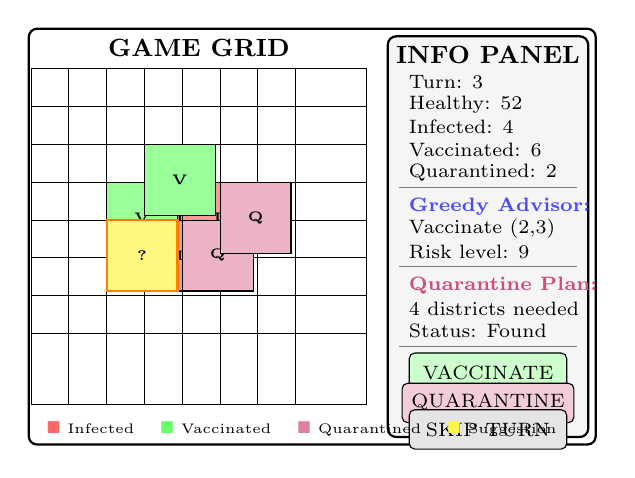
\begin{tikzpicture}[
  scale=0.48,
  cell/.style={draw, minimum size=0.9cm, inner sep=0pt, font=\tiny},
]
  % Main frame
  \draw[thick, rounded corners=3pt] (-0.5, -0.5) rectangle (14.5, 10.5);

  % Grid area label
  \node[font=\small\bfseries] at (4, 10) {GAME GRID};

  % 8x8 grid
  \foreach \r in {0,...,7} {
    \foreach \c in {0,...,7} {
      \node[cell, fill=white] at (\c+0.5, 8.5-\r) {};
    }
  }

  % Example colored cells
  \node[cell, fill=red!40]    at (3.5, 5.5) {\textbf{I}};
  \node[cell, fill=red!40]    at (4.5, 5.5) {\textbf{I}};
  \node[cell, fill=red!40]    at (3.5, 4.5) {\textbf{I}};
  \node[cell, fill=green!40]  at (2.5, 5.5) {\textbf{V}};
  \node[cell, fill=green!40]  at (3.5, 6.5) {\textbf{V}};
  \node[cell, fill=purple!30] at (4.5, 4.5) {\textbf{Q}};
  \node[cell, fill=purple!30] at (5.5, 5.5) {\textbf{Q}};

  % Highlight (greedy suggestion)
  \node[cell, fill=yellow!50, draw=orange, thick] at (2.5, 4.5) {\textbf{?}};

  % Side panel
  \draw[thick, fill=gray!8, rounded corners=3pt]
    (9, -0.3) rectangle (14.3, 10.3);
  \node[font=\small\bfseries] at (11.65, 9.8) {INFO PANEL};

  % Turn info
  \node[font=\scriptsize, anchor=west] at (9.3, 9.1) {Turn: 3};
  \node[font=\scriptsize, anchor=west] at (9.3, 8.5) {Healthy: 52};
  \node[font=\scriptsize, anchor=west] at (9.3, 7.9) {Infected: 4};
  \node[font=\scriptsize, anchor=west] at (9.3, 7.3) {Vaccinated: 6};
  \node[font=\scriptsize, anchor=west] at (9.3, 6.7) {Quarantined: 2};

  % Separator
  \draw[gray] (9.3, 6.3) -- (14.0, 6.3);

  % Greedy suggestion
  \node[font=\scriptsize\bfseries, anchor=west, text=blue!70]
    at (9.3, 5.8) {Greedy Advisor:};
  \node[font=\scriptsize, anchor=west] at (9.3, 5.2) {Vaccinate (2,3)};
  \node[font=\scriptsize, anchor=west] at (9.3, 4.6) {Risk level: 9};

  % Separator
  \draw[gray] (9.3, 4.2) -- (14.0, 4.2);

  % Backtracking result
  \node[font=\scriptsize\bfseries, anchor=west, text=purple!70]
    at (9.3, 3.7) {Quarantine Plan:};
  \node[font=\scriptsize, anchor=west] at (9.3, 3.1) {4 districts needed};
  \node[font=\scriptsize, anchor=west] at (9.3, 2.5) {Status: Found};

  % Separator
  \draw[gray] (9.3, 2.1) -- (14.0, 2.1);

  % Buttons
  \node[draw, rounded corners=2pt, fill=green!20, font=\scriptsize,
        minimum width=2cm, minimum height=0.5cm] at (11.65, 1.4)
    {VACCINATE};
  \node[draw, rounded corners=2pt, fill=purple!20, font=\scriptsize,
        minimum width=2cm, minimum height=0.5cm] at (11.65, 0.6)
    {QUARANTINE};
  \node[draw, rounded corners=2pt, fill=gray!20, font=\scriptsize,
        minimum width=2cm, minimum height=0.5cm] at (11.65, -0.1)
    {SKIP TURN};

  % Legend
  \node[font=\tiny, anchor=west] at (-0.3, -0.1) {
    \textcolor{red!60}{$\blacksquare$} Infected \quad
    \textcolor{green!60}{$\blacksquare$} Vaccinated \quad
    \textcolor{purple!50}{$\blacksquare$} Quarantined \quad
    \textcolor{yellow!70}{$\blacksquare$} Suggestion
  };

\end{tikzpicture}
\caption{Wireframe of the Pygame interface showing the grid, info panel, and
action buttons.}
\label{fig:wireframe}
\end{figure}

\subsection{Visual Encoding}

Each district state is represented by a distinct color on the grid:

\begin{itemize}
    \item \textbf{White} — healthy district.
    \item \textbf{Red} — infected district.
    \item \textbf{Green} — vaccinated district.
    \item \textbf{Purple} — quarantined district.
    \item \textbf{Yellow border} — district recommended by the greedy advisor.
\end{itemize}

Each cell also displays its risk level as a number (1--10) in the center, so
the player can make informed decisions.

\subsection{Player Interaction}

The player interacts with the game through three mechanisms:

\begin{enumerate}
    \item \textbf{Click on a grid cell} to select a district for vaccination.
          The selected cell is highlighted, and the side panel updates to show
          its risk level.
    \item \textbf{Click the VACCINATE button} to confirm vaccinating the
          selected district.
    \item \textbf{Click the QUARANTINE button} to accept the backtracking plan
          and quarantine all districts in the proposed set.
    \item \textbf{Click SKIP TURN} to pass without acting.
\end{enumerate}

After any action, the interface writes \texttt{action.json} and signals the
C++ engine to process the next turn.

\subsection{Detailed Wireframe}

Figure~\ref{fig:wireframe_detail} shows a more detailed wireframe that
includes the color legend, risk numbers inside each cell, and the side-panel
layout used during gameplay.

\begin{figure}[ht]
\centering
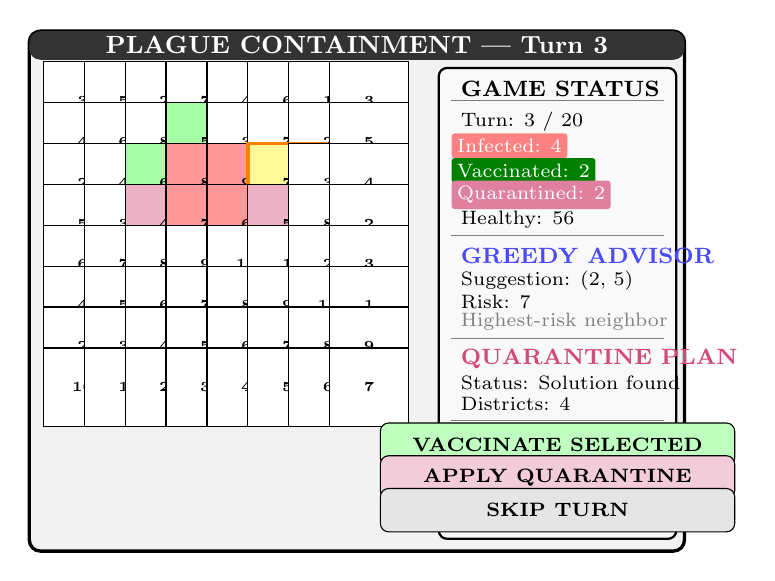
\begin{tikzpicture}[
  scale=0.52,
  cell/.style={draw, minimum size=1.0cm, inner sep=0pt,
               font=\tiny\bfseries},
]
  % Window border
  \draw[very thick, rounded corners=4pt, fill=black!5]
    (-0.8, -1.5) rectangle (15.2, 11.2);

  % Title bar
  \fill[black!80, rounded corners=4pt]
    (-0.8, 10.5) rectangle (15.2, 11.2);
  \node[font=\small\bfseries, text=white] at (7.2, 10.85)
    {PLAGUE CONTAINMENT --- Turn 3};

  % 8x8 grid with risk numbers
  % Row 0
  \node[cell, fill=white]      at (0.5, 9.5) {3};
  \node[cell, fill=white]      at (1.5, 9.5) {5};
  \node[cell, fill=white]      at (2.5, 9.5) {2};
  \node[cell, fill=white]      at (3.5, 9.5) {7};
  \node[cell, fill=white]      at (4.5, 9.5) {4};
  \node[cell, fill=white]      at (5.5, 9.5) {6};
  \node[cell, fill=white]      at (6.5, 9.5) {1};
  \node[cell, fill=white]      at (7.5, 9.5) {3};
  % Row 1
  \node[cell, fill=white]      at (0.5, 8.5) {4};
  \node[cell, fill=white]      at (1.5, 8.5) {6};
  \node[cell, fill=white]      at (2.5, 8.5) {8};
  \node[cell, fill=green!35]   at (3.5, 8.5) {5};
  \node[cell, fill=white]      at (4.5, 8.5) {3};
  \node[cell, fill=white]      at (5.5, 8.5) {7};
  \node[cell, fill=white]      at (6.5, 8.5) {2};
  \node[cell, fill=white]      at (7.5, 8.5) {5};
  % Row 2
  \node[cell, fill=white]      at (0.5, 7.5) {2};
  \node[cell, fill=white]      at (1.5, 7.5) {4};
  \node[cell, fill=green!35]   at (2.5, 7.5) {6};
  \node[cell, fill=red!40]     at (3.5, 7.5) {8};
  \node[cell, fill=red!40]     at (4.5, 7.5) {9};
  \node[cell, fill=yellow!40, draw=orange, very thick]
    at (5.5, 7.5) {7};
  \node[cell, fill=white]      at (6.5, 7.5) {3};
  \node[cell, fill=white]      at (7.5, 7.5) {4};
  % Row 3
  \node[cell, fill=white]      at (0.5, 6.5) {5};
  \node[cell, fill=white]      at (1.5, 6.5) {3};
  \node[cell, fill=purple!30]  at (2.5, 6.5) {4};
  \node[cell, fill=red!40]     at (3.5, 6.5) {7};
  \node[cell, fill=red!40]     at (4.5, 6.5) {6};
  \node[cell, fill=purple!30]  at (5.5, 6.5) {5};
  \node[cell, fill=white]      at (6.5, 6.5) {8};
  \node[cell, fill=white]      at (7.5, 6.5) {2};
  % Rows 4-7 (healthy)
  \foreach \r in {4,...,7} {
    \foreach \c in {0,...,7} {
      \pgfmathtruncatemacro{\riskval}{mod(\r*8+\c+3, 10)+1}
      \node[cell, fill=white] at (\c+0.5, 9.5-\r) {\riskval};
    }
  }

  % Side panel
  \draw[thick, fill=gray!5, rounded corners=3pt]
    (9.2, -1.2) rectangle (15.0, 10.3);

  % Stats
  \node[font=\footnotesize\bfseries, anchor=west] at (9.5, 9.8)
    {GAME STATUS};
  \draw[gray] (9.5, 9.5) -- (14.7, 9.5);
  \node[font=\scriptsize, anchor=west] at (9.5, 9.0) {Turn: 3 / 20};
  \node[font=\scriptsize, anchor=west, text=white, fill=red!50,
        rounded corners=1pt, inner sep=2pt] at (9.5, 8.4)
    { Infected: 4 };
  \node[font=\scriptsize, anchor=west, text=white, fill=green!50!black,
        rounded corners=1pt, inner sep=2pt] at (9.5, 7.8)
    { Vaccinated: 2 };
  \node[font=\scriptsize, anchor=west, text=white, fill=purple!50,
        rounded corners=1pt, inner sep=2pt] at (9.5, 7.2)
    { Quarantined: 2 };
  \node[font=\scriptsize, anchor=west] at (9.5, 6.6) {Healthy: 56};

  \draw[gray] (9.5, 6.2) -- (14.7, 6.2);

  % Advisor
  \node[font=\footnotesize\bfseries, anchor=west, text=blue!70]
    at (9.5, 5.7) {GREEDY ADVISOR};
  \node[font=\scriptsize, anchor=west] at (9.5, 5.1) {Suggestion: (2, 5)};
  \node[font=\scriptsize, anchor=west] at (9.5, 4.6) {Risk: 7};
  \node[font=\scriptsize, anchor=west, text=gray] at (9.5, 4.1)
    {Highest-risk neighbor};

  \draw[gray] (9.5, 3.7) -- (14.7, 3.7);

  % Quarantine plan
  \node[font=\footnotesize\bfseries, anchor=west, text=purple!70]
    at (9.5, 3.2) {QUARANTINE PLAN};
  \node[font=\scriptsize, anchor=west] at (9.5, 2.6)
    {Status: Solution found};
  \node[font=\scriptsize, anchor=west] at (9.5, 2.1) {Districts: 4};

  \draw[gray] (9.5, 1.7) -- (14.7, 1.7);

  % Action buttons
  \node[draw, rounded corners=3pt, fill=green!25,
        font=\scriptsize\bfseries, minimum width=4.5cm,
        minimum height=0.55cm] at (12.1, 1.1) {VACCINATE SELECTED};
  \node[draw, rounded corners=3pt, fill=purple!20,
        font=\scriptsize\bfseries, minimum width=4.5cm,
        minimum height=0.55cm] at (12.1, 0.3) {APPLY QUARANTINE};
  \node[draw, rounded corners=3pt, fill=gray!20,
        font=\scriptsize\bfseries, minimum width=4.5cm,
        minimum height=0.55cm] at (12.1, -0.5) {SKIP TURN};

\end{tikzpicture}
\caption{Detailed wireframe of the game interface. Each cell shows its risk
level. Colors encode district states. The yellow-bordered cell marks the greedy
suggestion.}
\label{fig:wireframe_detail}
\end{figure}

% ══════════════════════════════════════════════════════════════════════════════
\section{Conclusions}

This paper has presented the problem background and the complete design for
\emph{Plague Containment}. The city is modelled as an $8\times8$ grid where
each district carries a risk level and can be in one of four states. Two
algorithms drive the game mechanics: a greedy vaccination advisor that always
targets the highest-risk unprotected border district, and a backtracking
quarantine planner that exhaustively searches for a valid containment perimeter
while respecting the connectivity of the healthy city.

The system is organized in three layers — a C++ engine for data structures, a
Python module for algorithms, and a Pygame front-end for rendering and input —
connected through three JSON files (\texttt{state.json}, \texttt{result.json},
and \texttt{action.json}) that form a language-neutral communication bridge.

The next steps for the project are to implement both algorithms in Python,
build the Pygame interface, and develop the C++ engine that manages the game
state.


% ══════════════════════════════════════════════════════════════════════════════
% Pegar ANTES de \begin{thebibliography} en el documento principal.
% ══════════════════════════════════════════════════════════════════════════════

\section{Work Distribution}

Table~\ref{tab:workdist} describes the responsibility of each team member
during the Checkpoint phase. Each member contributed one major component of the
game design.

\begin{table}[ht]
\centering
\caption{Work distribution for the Checkpoint deliverable.}
\label{tab:workdist}
\begin{tabular}{|p{3.0cm}|p{1.2cm}|p{3.5cm}|}
\hline
\textbf{Team Member} & \textbf{Role} & \textbf{Deliverables} \\
\hline
Nelson David Molina Ramos &
Data Structures (C++) &
Design and diagrams of the infection linked list and the district-risk AVL
tree. Explanation of how each structure supports the game engine. \\
\hline
Brayan Estiven Aguirre Aristizabal &
Algorithms (Python) &
Pseudo-code and step-by-step explanation of the Greedy Vaccination algorithm
and the Backtracking Quarantine algorithm. \\
\hline
Juan Sneyder M\'{e}ndez Gil &
Interface \& Integration &
Pygame wireframe design, JSON schema specification
(\texttt{state.json}, \texttt{result.json}, \texttt{action.json}), and
system architecture describing how the C++ engine, Python algorithms, and
Pygame interface communicate. \\
\hline
\end{tabular}
\end{table}

All three components were designed to be consistent with each other: the JSON
fields map directly to the data structures defined by the engine developer, the
algorithm outputs match the fields read by the interface, and the wireframe
reflects the information provided by both the engine and the algorithms.



% ── References ────────────────────────────────────────────────────────────────
\begin{thebibliography}{00}

\bibitem{cormen2009introduction}
T.~H. Cormen, C.~E. Leiserson, R.~L. Rivest, and C.~Stein,
\textit{Introduction to Algorithms}, 3rd~ed.
Cambridge, MA: MIT Press, 2009.

\bibitem{russell2020artificial}
S.~Russell and P.~Norvig,
\textit{Artificial Intelligence: A Modern Approach}, 4th~ed.
Hoboken, NJ: Pearson, 2020.

\bibitem{pastor2015epidemic}
R.~Pastor-Satorras, C.~Castellano, P.~Van~Mieghem, and A.~Vespignani,
``Epidemic processes in complex networks,''
\textit{Reviews of Modern Physics}, vol.~87, no.~3, pp.~925--979, 2015.

\end{thebibliography}

\end{document}

\end{document}